\documentclass[12pt]{article}
\usepackage[margin=2.5cm]{geometry}
\usepackage{enumerate}
\usepackage{amsfonts}
\usepackage{amsmath}
\usepackage{fancyhdr}
\usepackage{amsmath}
\usepackage{amssymb}
\usepackage{amsthm}
\usepackage{mdframed}
\usepackage{graphicx}
\usepackage{subcaption}
\usepackage{adjustbox}
\usepackage{listings}
\usepackage{xcolor}
\usepackage{soul}
\usepackage{booktabs}
\usepackage[utf]{kotex}
\usepackage{hyperref}

\definecolor{codegreen}{rgb}{0,0.6,0}
\definecolor{codegray}{rgb}{0.5,0.5,0.5}
\definecolor{codepurple}{rgb}{0.58,0,0.82}
\definecolor{backcolour}{rgb}{0.95,0.95,0.92}

\lstdefinestyle{mystyle}{
    backgroundcolor=\color{backcolour},
    commentstyle=\color{codegreen},
    keywordstyle=\color{magenta},
    numberstyle=\tiny\color{codegray},
    stringstyle=\color{codepurple},
    basicstyle=\ttfamily\footnotesize,
    breakatwhitespace=false,
    breaklines=true,
    captionpos=b,
    keepspaces=true,
    numbers=left,
    numbersep=5pt,
    showspaces=false,
    showstringspaces=false,
    showtabs=false,
    tabsize=1
}

\lstset{style=mystyle}

\pagestyle{fancy}
\renewcommand{\headrulewidth}{0.4pt}
\lhead{CSC 373}
\rhead{Worksheet 6 Solution}

\begin{document}
\title{CSC373 Worksheet 6 Solution}
\maketitle

\bigskip

\begin{enumerate}[1.]
    \item

    \begin{enumerate}[1.]
        \item Multiply objective function by - 1

        \bigskip

        \begin{mdframed}

        Maximize

        \begin{align*}
            -2x_1 - 7x_2 - x_3
        \end{align*}

        Subject to

        \begin{align*}
            x_1 - x_3  &= 7\\
            3x_1 + x_2 &\geq 7\\
            x_2 &\geq 0\\
            x_3 &\leq 0
        \end{align*}

        \end{mdframed}

        \item Replace non-nonnegative constraints $x_1$

        \begin{mdframed}

        Maximize

        \begin{align*}
            -2x_1' + 2x_1'' - 7x_2 - x_3
        \end{align*}

        Subject to

        \begin{align*}
            x_1' - x_1'' - x_3  &= 7\\
            3x_1' - 3x_1'' + x_2 &\geq 7\\
            x_1', x_1'', x_2 &\geq 0\\
            x_3 &\leq 0
        \end{align*}

        \end{mdframed}

        \item Replace non-nonnegative constraints $x_3$

        \begin{mdframed}

        Maximize

        \begin{align*}
            -2x_1' + 2x_1'' - 7x_2 - x_3' + x_3''
        \end{align*}

        Subject to

        \begin{align*}
            x_1' - x_1'' - x_3' + x_3''  &= 7\\
            3x_1' - 3x_1'' + x_2 &\geq 7\\
            x_1', x_1'', x_2, x_3', x_3'' &\geq 0\\
        \end{align*}

        \end{mdframed}

        \item Replace equality constraints with $\geq$ and $\leq$

        \begin{mdframed}

        Maximize

        \begin{align*}
            -2x_1' + 2x_1'' - 7x_2 - x_3' + x_3''
        \end{align*}

        Subject to

        \begin{align*}
            x_1' - x_1'' - x_3' + x_3''  &\leq 7\\
            x_1' - x_1'' - x_3' + x_3''  &\geq 7\\
            3x_1' - 3x_1'' + x_2 &\geq 7\\
            x_1', x_1'', x_2, x_3', x_3'' &\geq 0\\
        \end{align*}

        \end{mdframed}

        \item Correct greater-than-or-equal-to inequality constraints

        \begin{mdframed}

        Maximize

        \begin{align*}
            -2x_1' + 2x_1'' - 7x_2 - x_3' + x_3''
        \end{align*}

        Subject to

        \begin{align*}
            x_1' - x_1'' - x_3' + x_3''  &\leq 7\\
            -x_1' + x_1'' + x_3' - x_3''  &\leq -7\\
            -3x_1' + 3x_1'' - x_2 &\leq 7\\
            x_1', x_1'', x_2, x_3', x_3'' &\geq 0\\
        \end{align*}


        \end{mdframed}
    \end{enumerate}

    % \bigskip

    % \underline{\textbf{Rough Works:}}

    % \begin{enumerate}[1.]
    %     \item Multiply objective function by - 1

    %     \bigskip

    %     \begin{mdframed}

    %     Maximize

    %     \begin{align*}
    %         -2x_1 - 7x_2 - x_3
    %     \end{align*}

    %     Subject to

    %     \begin{align*}
    %         x_1 - x_3  &= 7\\
    %         3x_1 + x_2 &\geq 7\\
    %         x_2 &\geq 0\\
    %         x_3 &\leq 0
    %     \end{align*}

    %     \end{mdframed}

    %     \item Replace non-nonnegative constraints $x_1$

    %     \begin{mdframed}

    %     Maximize

    %     \begin{align*}
    %         -2x_1' + 2x_1'' - 7x_2 - x_3
    %     \end{align*}

    %     Subject to

    %     \begin{align*}
    %         x_1' - x_1'' - x_3  &= 7\\
    %         3x_1' - 3x_1'' + x_2 &\geq 7\\
    %         x_1', x_1'', x_2 &\geq 0\\
    %         x_3 &\leq 0
    %     \end{align*}

    %     \end{mdframed}

    %     \item Replace non-nonnegative constraints $x_3$

    %     \begin{mdframed}

    %     Maximize

    %     \begin{align*}
    %         -2x_1' + 2x_1'' - 7x_2 - x_3' + x_3''
    %     \end{align*}

    %     Subject to

    %     \begin{align*}
    %         x_1' - x_1'' - x_3' + x_3''  &= 7\\
    %         3x_1' - 3x_1'' + x_2 &\geq 7\\
    %         x_1', x_1'', x_2, x_3', x_3'' &\geq 0\\
    %     \end{align*}

    %     \end{mdframed}

    %     \item Replace equality constraints with $\geq$ and $\leq$

    %     \begin{mdframed}

    %     Maximize

    %     \begin{align*}
    %         -2x_1' + 2x_1'' - 7x_2 - x_3' + x_3''
    %     \end{align*}

    %     Subject to

    %     \begin{align*}
    %         x_1' - x_1'' - x_3' + x_3''  &\leq 7\\
    %         x_1' - x_1'' - x_3' + x_3''  &\geq 7\\
    %         3x_1' - 3x_1'' + x_2 &\geq 7\\
    %         x_1', x_1'', x_2, x_3', x_3'' &\geq 0\\
    %     \end{align*}

    %     \end{mdframed}

    %     \item Correct greater-than-or-equal-to inequality constraints

    %     \begin{mdframed}

    %     Maximize

    %     \begin{align*}
    %         -2x_1' + 2x_1'' - 7x_2 - x_3' + x_3''
    %     \end{align*}

    %     Subject to

    %     \begin{align*}
    %         x_1' - x_1'' - x_3' + x_3''  &\leq 7\\
    %         -x_1' + x_1'' + x_3' - x_3''  &\leq -7\\
    %         -3x_1' + 3x_1'' - x_2 &\leq 7\\
    %         x_1', x_1'', x_2, x_3', x_3'' &\geq 0\\
    %     \end{align*}


    %     \end{mdframed}
    % \end{enumerate}

    \bigskip

    \underline{\textbf{Notes:}}

    \bigskip

    \begin{itemize}
        \item \textbf{Linear Programming}
        \begin{itemize}
            \item Is a method to achieve the best outcome (such as maximum profit or lowest cost) in a mathematical model
            whose requirements are represented by linear relationships. $^{[1]}$
            \item Is named to make it sound cool for government funding
            \begin{itemize}
                \item Like dynamic programming
            \end{itemize}
            \item Applications

            \begin{itemize}
                \item Microeconomics (maximize profits, minimize costs)
                \item Company management
            \end{itemize}
        \end{itemize}

        \item \textbf{Standard Form}

        \begin{itemize}
            \item Is a form of linear programming
            \item Are about \ul{maximizing}, not minimizing $^{[2]}$
            \item All have a positivity constraint for each variable $^{[2]}$
            \item All other constraints are all of the form “linear combination of variables $\leq$ constant”. $^{[2]}$
        \end{itemize}

        \bigskip

        \begin{center}
        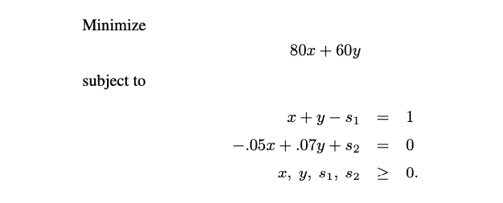
\includegraphics[width=0.8\linewidth]{images/worksheet_6_solution_1.png}
        \end{center}

        \item \textbf{Converting Linear Programming to Standard Form}

        \begin{enumerate}[1)]
            \item The objective function might be a minimization rather than a maximization

            \begin{itemize}
                \item Negate coefficients of the objective function
            \end{itemize}

            \begin{center}
            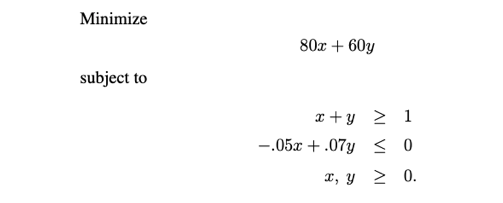
\includegraphics[width=0.9\linewidth]{images/worksheet_6_solution_2.png}
            \end{center}

            \item There might be variables without nonnegativity constraints

            \begin{itemize}
                \item Replace each non-nonnegative variable $x_i$ with $x_i'$ and $x_i''$
                \item Modify linear program
            \end{itemize}

            \begin{center}
            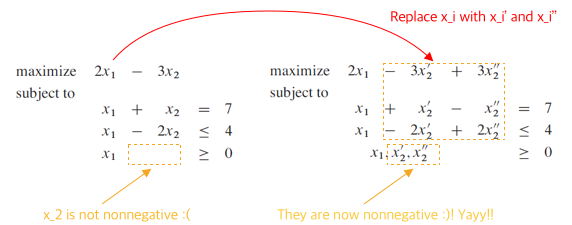
\includegraphics[width=0.9\linewidth]{images/worksheet_6_solution_3.png}
            \end{center}

            \item There might be \textbf{equality constraints}, which have an equal sign rather than a
            less-than-or-equal-to sign

            \begin{itemize}
                \item Replace equality constraint $f(x_1, x_2, ..., x_n) = b$ with
                $f(x_1, x_2, ..., x_n) \leq b$ and $f(x_1, x_2, ..., x_n) \geq b$
            \end{itemize}

            \begin{center}
            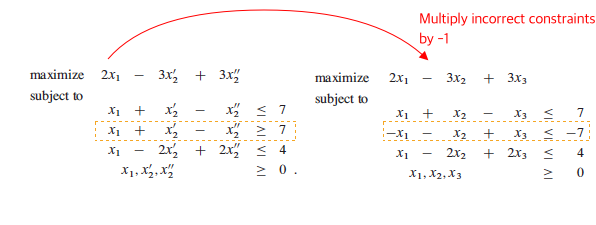
\includegraphics[width=0.9\linewidth]{images/worksheet_6_solution_5.png}
            \end{center}

            \item There might be \textbf{inequality constraints}, but instead of having a less-than-or-equal-to-sign

            \begin{itemize}
                \item Multiply incorrect inequality constraints by -1
            \end{itemize}

            \begin{center}
            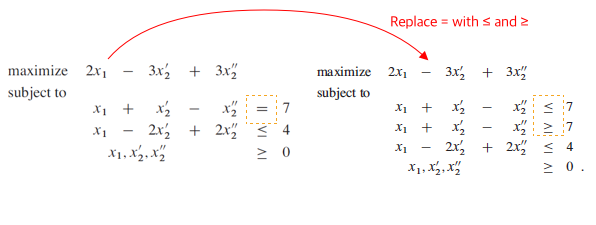
\includegraphics[width=0.9\linewidth]{images/worksheet_6_solution_4.png}
            \end{center}


        \end{enumerate}

    \end{itemize}

    \bigskip

    \underline{\textbf{References:}}

    \bigskip

    \begin{enumerate}[1)]
        \item Wikipedia, Linear Programming, \href{https://en.wikipedia.org/wiki/Linear_programming}{link}
        \item Instituto de Mathematicas, Standard form for Linear Programs, \href{https://www.matem.unam.mx/~omar/math340/std-form.html}{link}
    \end{enumerate}

    \item

    \bigskip

    \underline{\textbf{Notes:}}

    \bigskip

    \begin{itemize}

        \item \textbf{Slack Form}

        \begin{itemize}
            \item Is a form of linear programming
            \item Is for efficient solving of liner programming problem using simplex algorithm
        \end{itemize}

        \begin{center}
        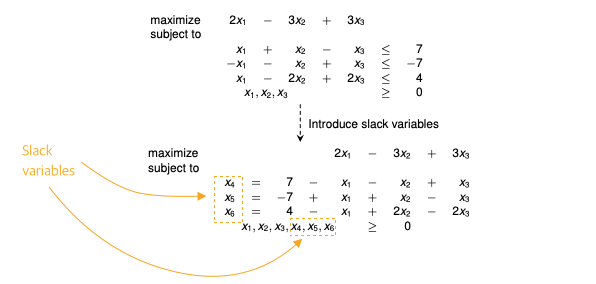
\includegraphics[width=\linewidth]{images/worksheet_6_solution_6.png}
        \end{center}
        \item \textbf{Converting Linear Programs into Slack Form}

        \begin{enumerate}[1)]
            \item Start from the standard form of linear programming
            \item Shift objective functions to right

            \begin{center}
            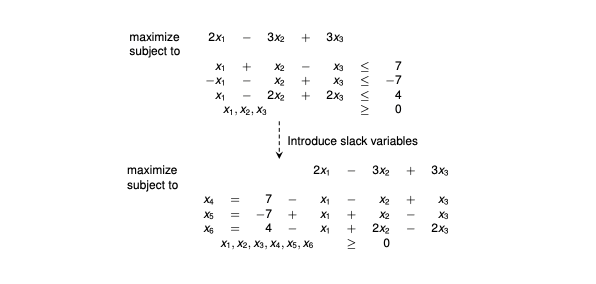
\includegraphics[width=\linewidth]{images/worksheet_6_solution_7.png}
            \end{center}

            \item Introduce slack variable $x_i$ to lhs and move expressions $\sum\limits_{j=1}^n a_{ij}x_j$ to rhs
            \item Change inequalities in linear programming to equality

            \begin{center}
            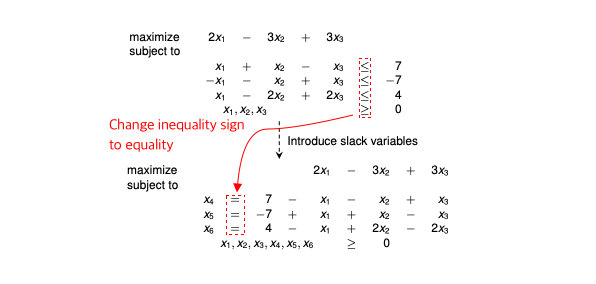
\includegraphics[width=\linewidth]{images/worksheet_6_solution_9.png}
            \end{center}

            \item Use Variable $z$ to denote objective function
            \item Omit the nonnegativivty constraints

            \begin{center}
            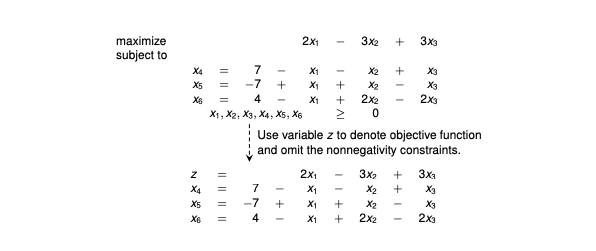
\includegraphics[width=\linewidth]{images/worksheet_6_solution_11.png}
            \end{center}
        \end{enumerate}
    \end{itemize}

    \bigskip

    \underline{\textbf{References:}}

    \bigskip

    \begin{enumerate}[1)]
        \item Cambridge University, Linear Programming, \href{https://www.cl.cam.ac.uk/teaching/1617/AdvAlgo/lp.pdf}{link}
    \end{enumerate}
\end{enumerate}

\end{document}